\documentclass{article}
\usepackage[T1]{fontenc}
\usepackage[utf8]{inputenc}
\usepackage[french]{babel}
\usepackage{listings, xcolor, graphicx}
\usepackage{amsmath}
\usepackage{textgreek}
\usepackage{enumitem}
\usepackage{subcaption}
\graphicspath{ {./} }

\title{Modélisation de la propagation des variants du COVID}
\author{BOUZAKRI Wassim \\COUPET Joss \\MARCHETTI Marie-Eden \\VASSEUR Pierre-Adrien}
\date{Février 2022}

\begin{document}

\maketitle

\section{Résumé}

Cet article s'intéresse à la problématique suivante : le comportement de l'épidémie de la COVID-19 est-il influencé par la circulation, la mutation et l'interaction de variants ?
Pour répondre à cette question, un certain nombre d'équations mathématiques ont été mises en place afin de réaliser un outil capable de modéliser ce problème. Grâce à cet outil, des simulations ont été faites. \\
Les analyses de ces simulations ont permis de conclure que la mutation et la virulence des variants influencent le comportement de l'épidémie. Les paramètres des variants initiaux sont particulièrement importants.

\section{Introduction}

Dans ce rapport, on va étudier la propagation de la COVID-19 par le biais des variants.
On se demande alors si leur circulation et mutation influencent le comportement de l'épidémie, en plus de considérer leur interaction entre eux.\\
\noindent
Concernant les recherches existantes, on a découvert peu d'articles présentant des simulations de propagation de la Covid-19 par le biais des variants.
Les quelques articles existants se concentraient surtout des propriétés biologiques du virus influençant la simulation de la mutation et la propagation.
Par exemple, la taille du génome du virus parent ou les symptômes. (Marquioni \& de Aguiar, 2021), ce sont des analyses intéressantes mais sans doute trop complexe sans avoir suivi la formation adéquate.\\
\noindent
Une approche différente et plus simple a été choisie afin de permettre la compréhension par un maximum de lecteurs. Elle sere détaillée tout au long de cet article.\\
\noindent
Tout d'abord, on présentera la modélisation de départ de la propagation de la Covid-19 initialisée avec un seul variant. \par
\noindent
Ensuite, on se penchera sur la modélisation plus complexe initialisée avec deux variants, sur laquelle on concentrera notre étude.\par
\noindent
Puis, on réalisera plusieurs simulations différentes dans l'objectif d'interpréter le comportement de ce modèle grâce aux résultats.\par
\noindent
Enfin, on conclura notre étude.\\

\section{Modélisation de départ}

La modélisation de départ est très basique et représente l'évolution d'un seul variant en prenant en compte sa virulence et sa force de contagion.\\
\noindent
Les variables de base pour seulement 1 virus sont les suivantes :
\begin{align}
    S(t)= \text{\% de personnes saines dans la population au temps t} \\
    I(t)= \text{\% de personnes contaminées dans la population au temps t} \\
    R(t)= \text{\% de personnes en rémission dans la population au temps t}
\end{align}
\noindent
\textalpha \space représente la force de contagion du virus. (quantité de virus / mL) \\
\textbeta \space représente la virulence du virus. (\% de survie) \\
\noindent
La simulation discrétisée par le temps est représentée dans le système d'équations suivantes :
\begin{align}
    \dot{S}(t)= -\alpha S(t)I(t) \\
    \dot{I}(t)= \alpha S(t)I(t)-\beta I(t) \\
    \dot{R}(t)= \beta I(t)
\end{align}
\noindent
Cette mise en équation permet de simuler facilement la propagation de la Covid-19 au sein d'une population saine.\\

\section{Modélisation avancée}

Afin de modéliser un modèle à X variants, un nouveau système d'équations est nécessaire.\\
Pour débuter, on a défini un nouveau modèle avec 2 variants qui pourra être modifié pour permettre de simuler X variants.\\
\noindent
Les variables de notre nouveau modèle sont les mêmes que précédemment, c'est-à-dire :
\begin{align}
    S_1(t)= \text{\% de non infecté par le variant 1.} \\
    S_2(t)= \text{\% de non infecté par le variant 2.} \\
    I_1(t)= \text{\% d'infecté au variant 1.} \\
    I_2(t)= \text{\% d'infecté au variant 2.} \\
    R_1(t)= \text{\% de remis au variant 1.} \\
    R_2(t)= \text{\% de remis au variant 2.}
\end{align}
\noindent
On obtient donc 2 systèmes d'équations différents. \\
\noindent
Le premier système d'équations est celui qui permet de simuler l'évolution du premier variant.\\
\begin{align}
    \dot{S_1}(t)= -\alpha_1 S_1(t)I_1(t) \\
    \dot{I_1}(t)= \alpha_1 S_1(t)I_1(t)-\beta_1 I_1(t) \\
    \dot{R_1}(t)= \beta_1 I_1(t)
\end{align}
On obtient le même pour le second variant. \\
Cependant le système est trop simple, il n'y a pas d'interaction entre les virus. \\
On fait donc un nouveau système qui permet une interaction entre les variants et qui sera adaptable à X variants à l'aide de boucles en programmation :
\begin{align}
    \dot{S}(t)= -\alpha_1 S(t)I_1(t) - \alpha_2 S(t)I_2(t) \\
    \dot{I_1}(t)= \alpha_1 S(t)I_1(t)-\beta_1 I_1(t) \\
    \dot{I_2}(t)= \alpha_2 S(t)I_2(t)-\beta_2 I_2(t) \\
    \dot{R}(t)= \beta_1 I_1(t) + \beta_2 I_2(t)
\end{align}
\noindent
Lors de la création de ce modèle, on a défini les règles suivantes :
\begin{enumerate}
    \item On ne peut être infecté que par un variant à la fois.
    \item Après s'être remis, on ne peut plus être infecté par un variant.
\end{enumerate}

\noindent
On veut maintenant modéliser les mutations.\\
Le \% de chance de mutation du variant 1 sur l'intervalle de temps T est définie par :
\begin{align}
    m = (1-e^{\gamma T})I_1(t) \text{ avec }\gamma > \text{0}
\end{align}
\noindent
Si une mutation doit être réalisée alors \\
\noindent
X est un nombre aléatoire tel que 0 < X < 100 \\
x est la probabilité que les propriétés d'un variant soient fortement différentes des propriétés du parent.\\
Si X > x \\
Alors F(X) =
\begin{align}
    n_\alpha \in \text{ ]}1.2\alpha_{variant}, 1.4\alpha_{variant}\text{[}  \\
    n_\beta \in \text{ ]}0.9\beta_{variant}, 1.1\beta_{variant}\text{[}
\end{align}
\noindent
Sinon F(X) = \\
\begin{align}
    n_\alpha \in \text{ ]}0.1\alpha_{variant}, 1.9\alpha_{variant}\text{[} \\
    n_\beta \in \text{ ]}0.1\beta_{variant}, 1.9\beta_{variant}\text{[}
\end{align}


\section{Simulations numériques}

Dans cette partie, on va réaliser plusieurs simulations avec différents paramètres. Ces simulations sont produites avec un outil que l'on a développé et déployé en ligne, disponible à l'adresse suivante : https://modelisation.vercel.app/ \\
Sur cet outil de modélisation, il est possible de choisir 2 types de représentation, une représentation en ligne et une représentation en pile (stack). Pour les simulations suivantes, nous avons décidé d'utiliser la représentation en ligne. \\
Les paramètres initiaux sont les suivants :
\begin{enumerate}
    \item Taux de personnes saines = 0,97
    \item Taux de personnes en rémission = 0
    \item Taux de mutabilité du virus = 0,01
    \item Probabilité de créer un nouveau variant avec des paramètres très éloignés de son parent = 1
    \item Durée de la simulation en jours = 2000 \\
\end{enumerate}
Pour le variant 1 :
\begin{enumerate}
    \item Taux de personnes infecté = 0,01
    \item Force de contagion du variant (quantité de virus / mL) = 0,01
    \item Virulence du variant (\% de survie) = 0,001\\
\end{enumerate}
Pour le variant 2 :
\begin{enumerate}
    \item Taux de personnes infecté = 0,02
    \item Force de contagion du variant (quantité de virus / mL) = 0,01
    \item Virulence du variant (\% de survie) = 0,005\\
\end{enumerate}


\noindent
La virulence d'un variant est un pourcentage de survie où plus le chiffre est proche de 0, plus la survie de l'infecter est faible.
Dans la majorité des simulations, on fera varier un seul de ces paramètres afin d'identifier la cause réelle du changement. \\
Si on se permet de modifier plusieurs paramètres en même temps, on ne peut plus être sûr de ce qui cause un possible changement observé. \\
\noindent
De plus, on remarque que les nouveaux variants entrainent une coupure dans les courbes des variants dont ils sont issus. \\
En effet, le taux de personnes infectées par un variant est issu du taux de personnes infectées par le variant parent. \\
Nous avons décidé de faire en sorte que la création d'un variant affecte un grand nombre de la population du variant parent afin d'avoir des résultats intéressants directement. Si nous avions décidé de faire muter qu'une petite partie de notre population, nous aurions eu des difficultés à étudier le développement des variants. En effet, dans la réalité, il y a des millions de variants qui naissent chaque jour mais seulement un faible nombre survit. Pour des raisons de performances, nous ne pouvons pas modéliser des millions de variants.

\subsection{Simulation de référence}

\begin{figure}[h]
    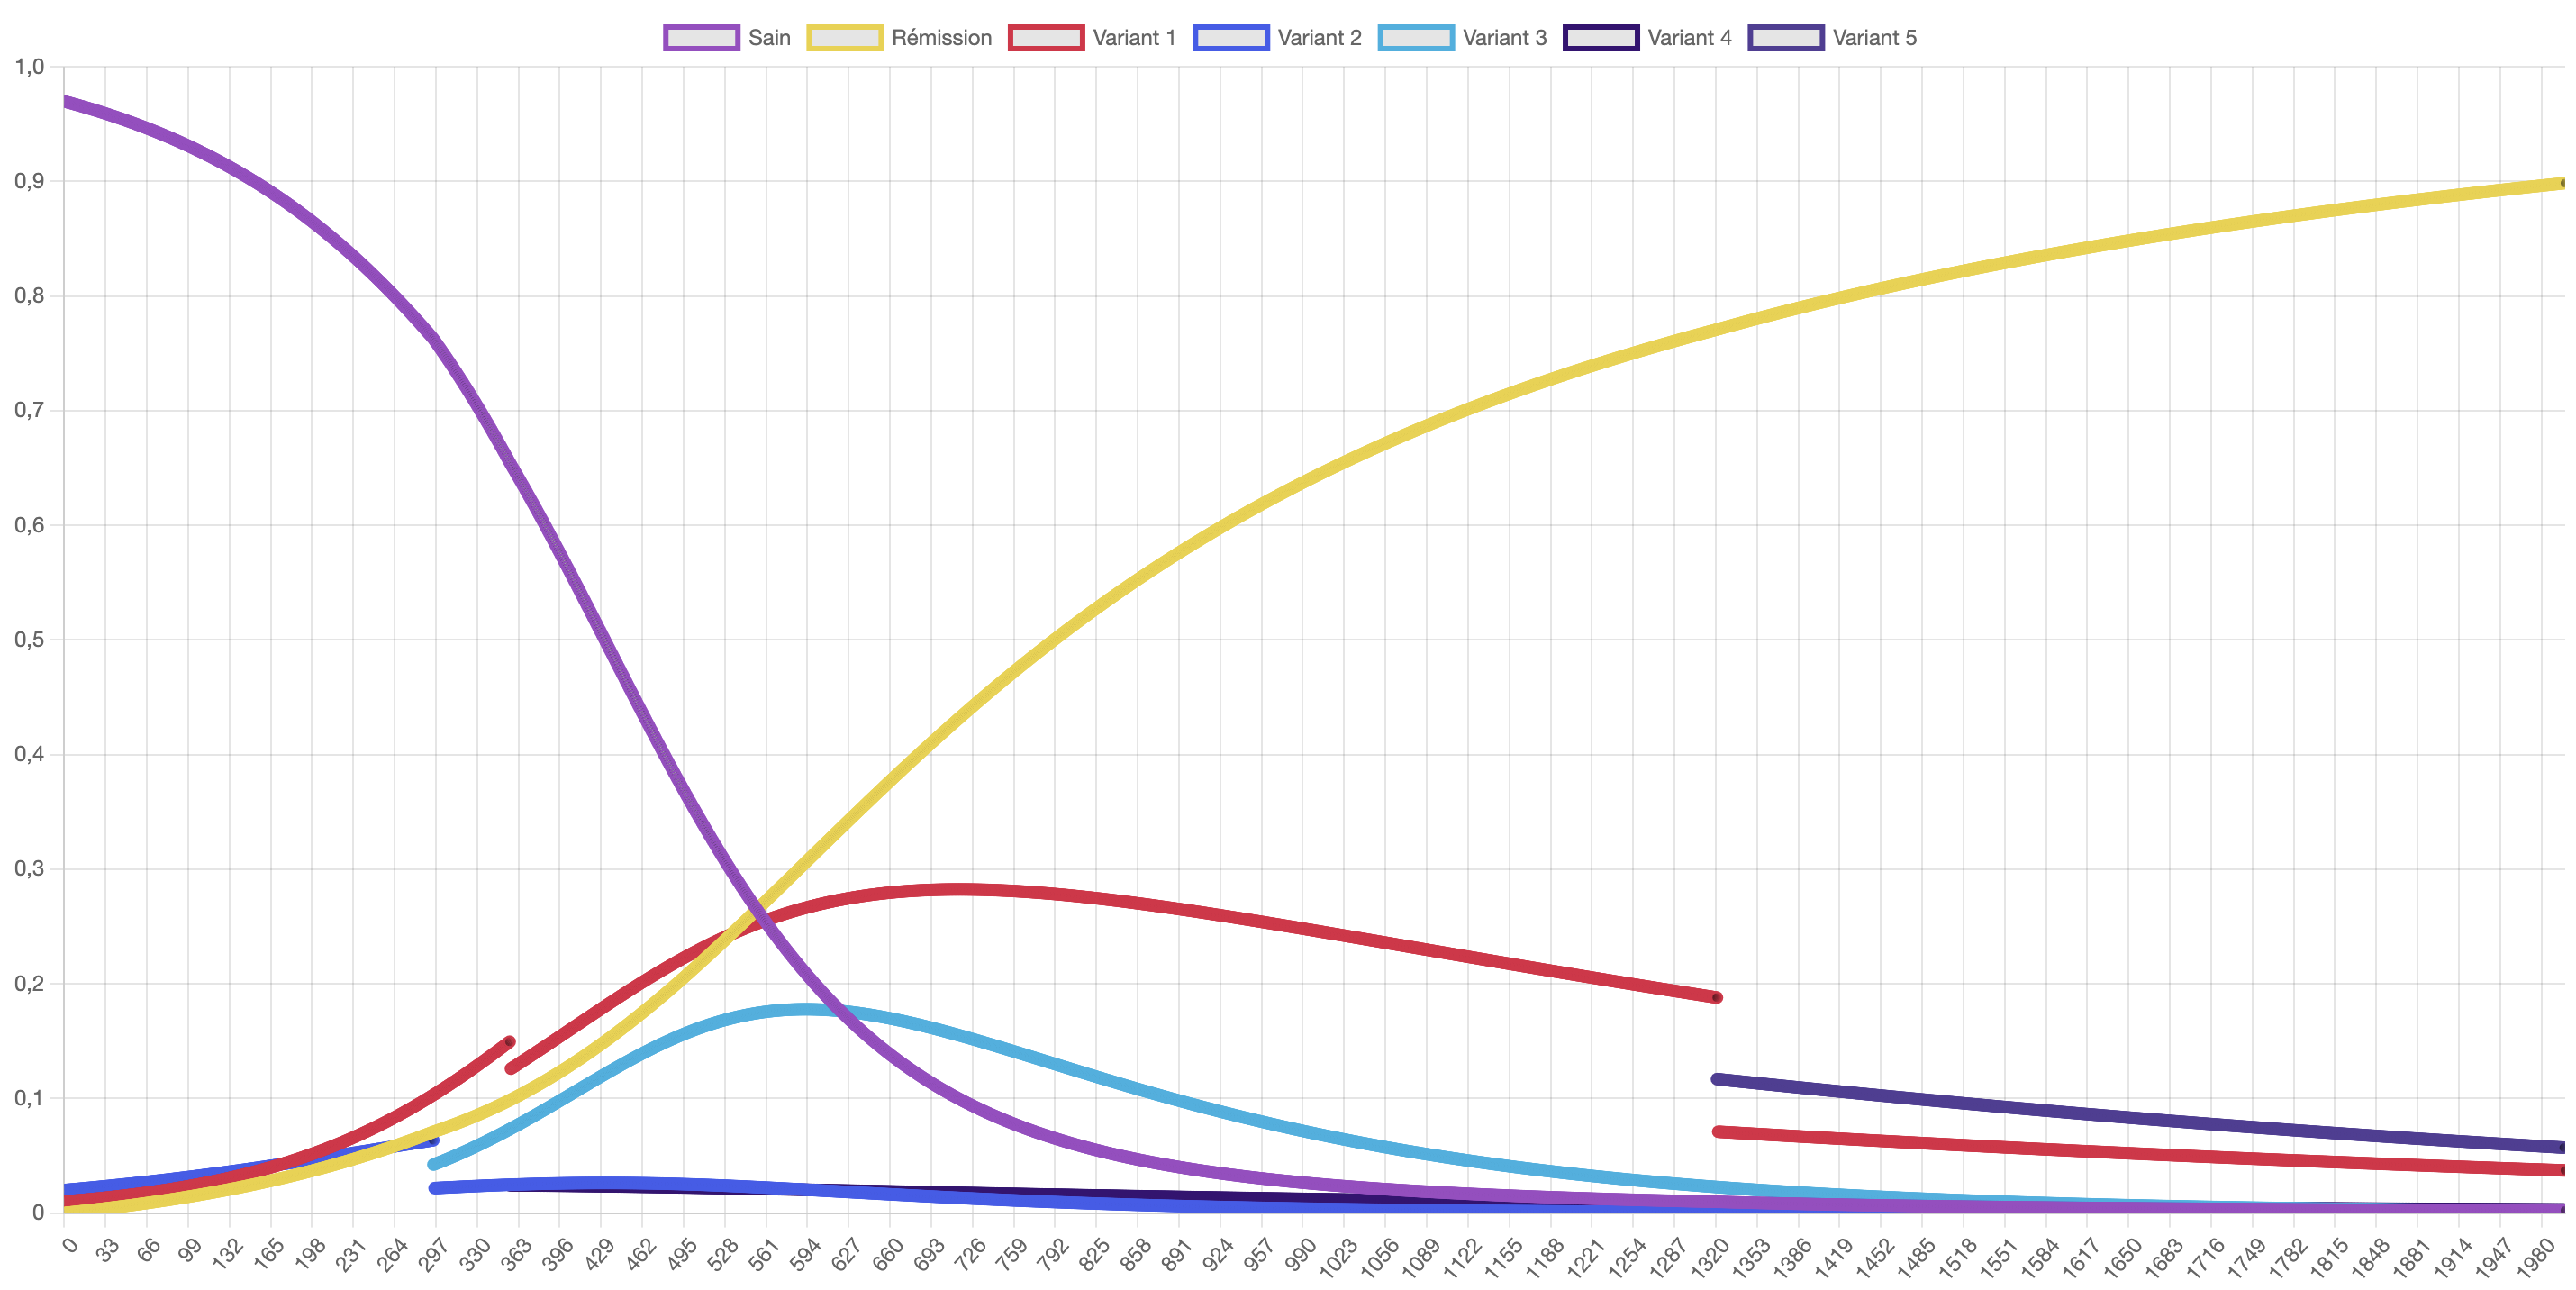
\includegraphics[width=\linewidth]{images/Simulation1.png}
    \caption{Simulation de référence}
    \label{fig:simulation1}
\end{figure}

\noindent
La simulation de référence utilise les paramètres de base énoncée un peu plus haut. \\
On remarque la création de 6 nouveaux variants :
\begin{enumerate}
    \item Variant 3 : Apparition au jour 231. Il est issu du variant 2. Il ne survit pas.
    \item Variant 4 : Apparition au jour 561. Il est issu du variant 1.
    \item Variant 5 : Apparition au jour 627. Il est issu du variant 4. Il survit avec un faible taux d'infection.
    \item Variant 6 : Apparition au jour 660. Il est issu du variant 2. Il ne survit pas.
    \item Variant 7 : Apparition au jour 1419. Il est issu du variant 4. Il ne survit pas.
    \item Variant 8 : Apparition dans les derniers jours de la modélisation.
\end{enumerate}
\noindent
La simulation de référence montre que l'on a une forte création de variant se basant sur le variant 1. En effet le variant 1 prend complètement le dessus sur le variant 2 alors qu'il possède un taux d'infecté inférieur au début de la simulation. Cela est dû au fait que le variant 1 est plus virulent. Ce dernier devient donc le variant à l'origine de tous les autres variants.

\subsection{Influence de la mutabilité du virus}

\begin{figure}[h]
  \begin{subfigure}{.5\textwidth}
  \centering
  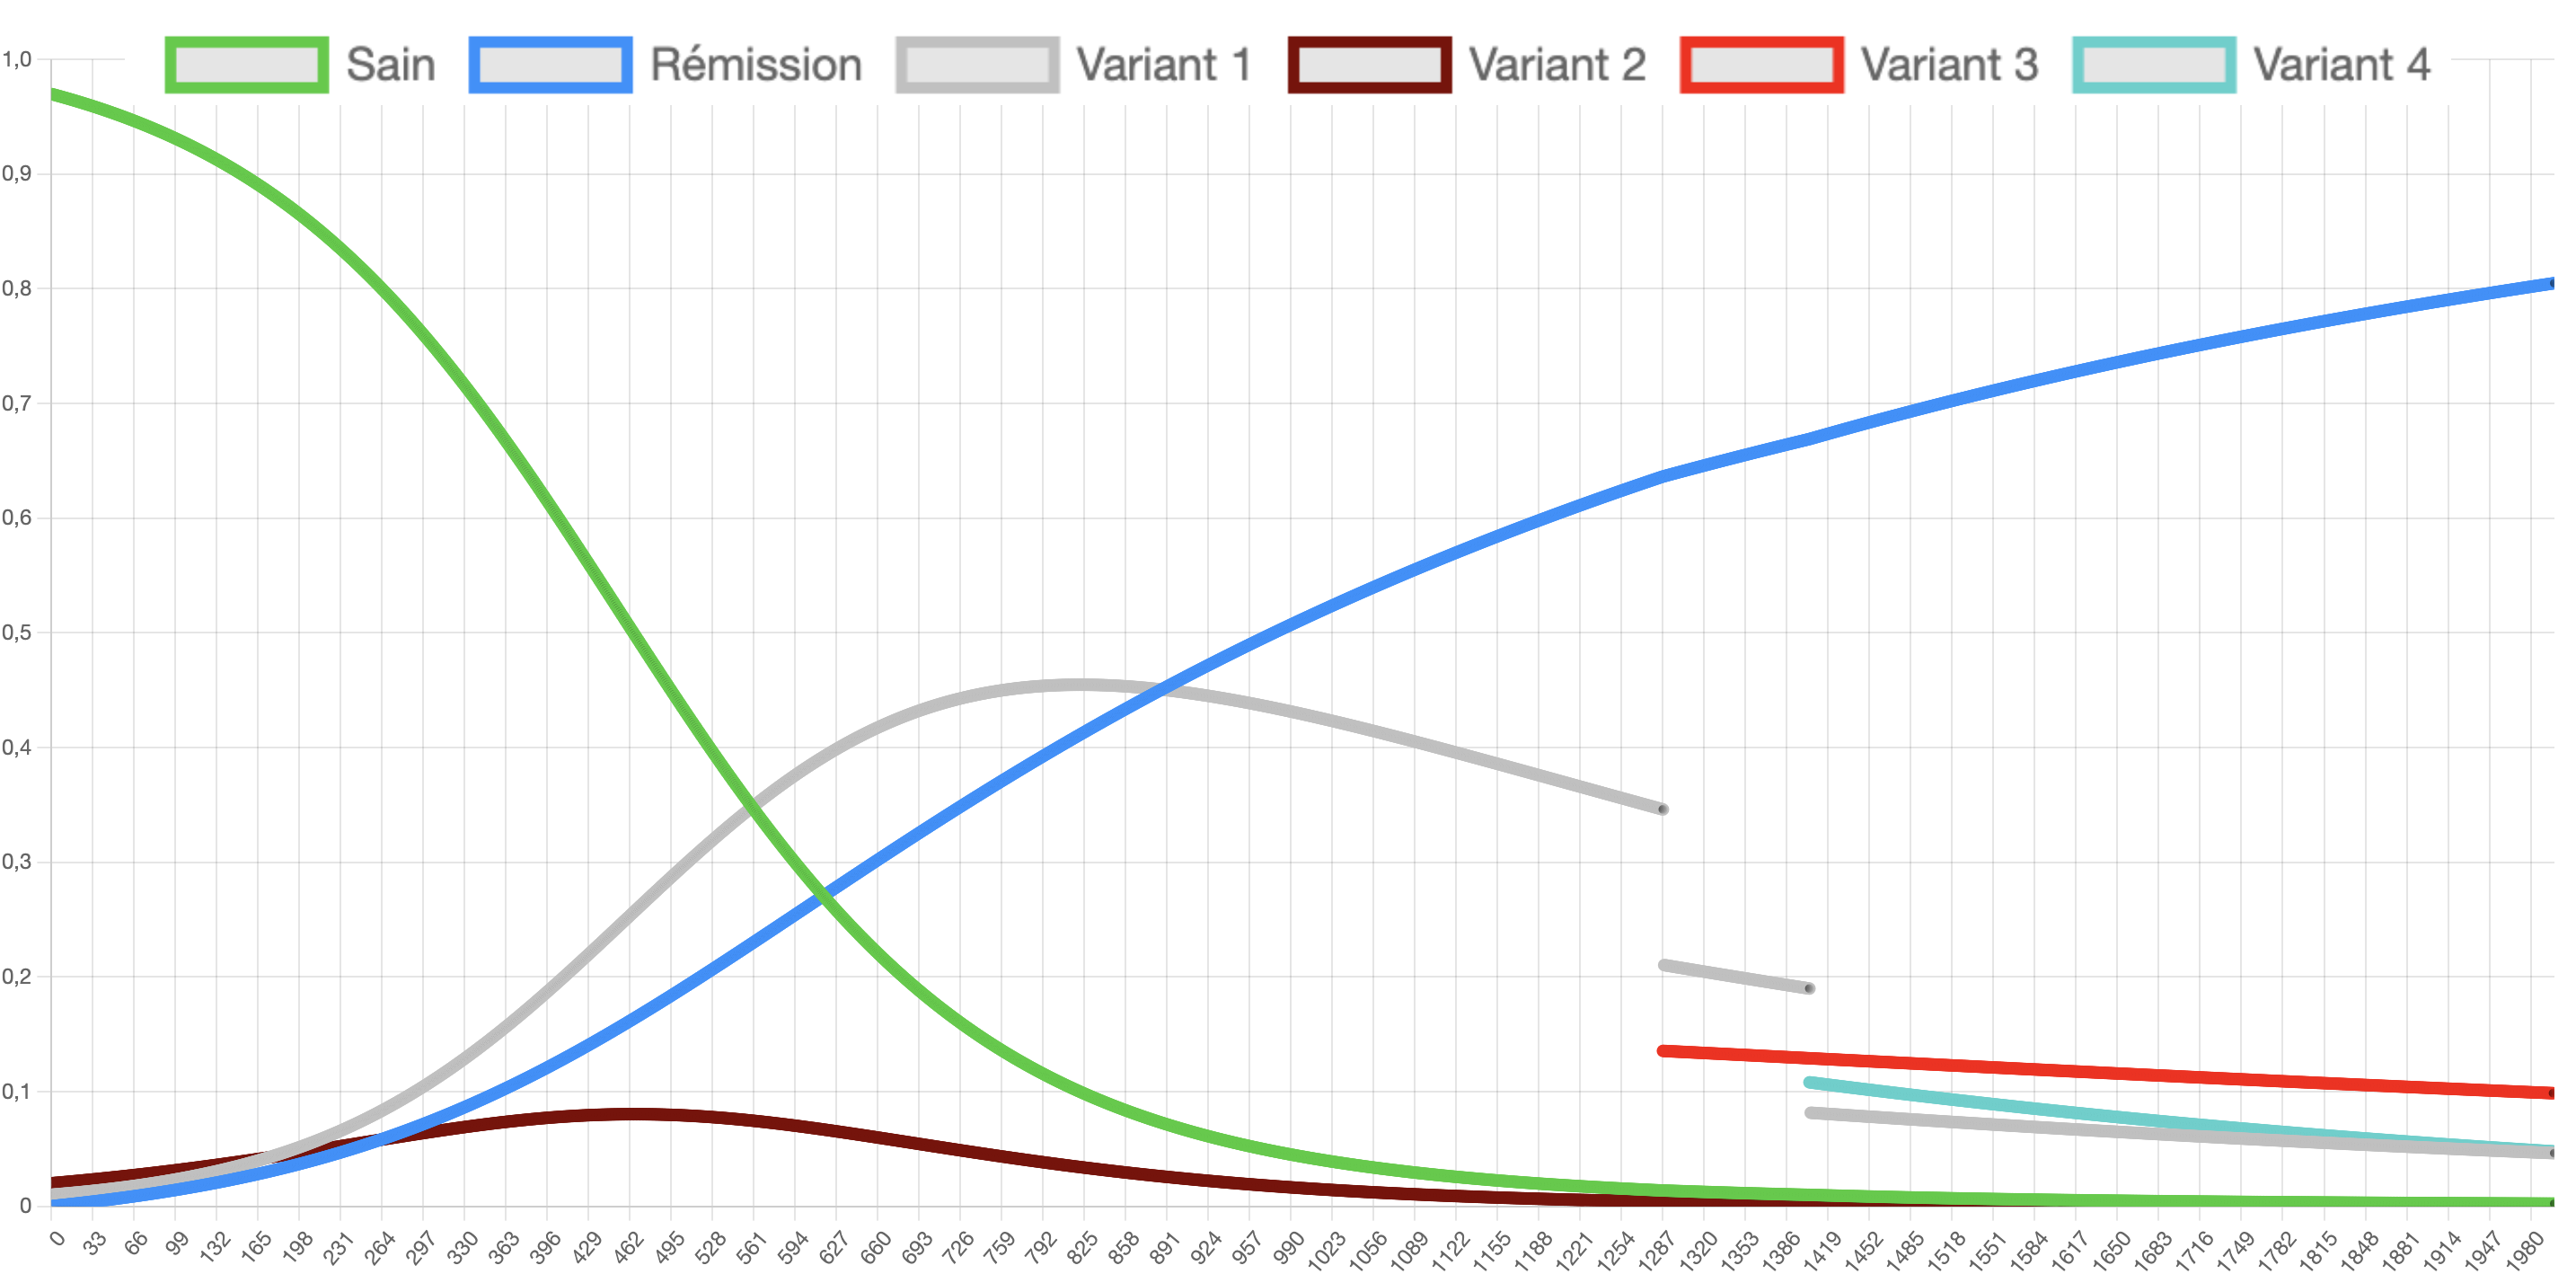
\includegraphics[width=1\linewidth]{images/Simulation2_1.png}
  \caption{Mutabilité du virus plus faible}
  \label{fig:sub1}
\end{subfigure}%
\begin{subfigure}{.5\textwidth}
  \centering
  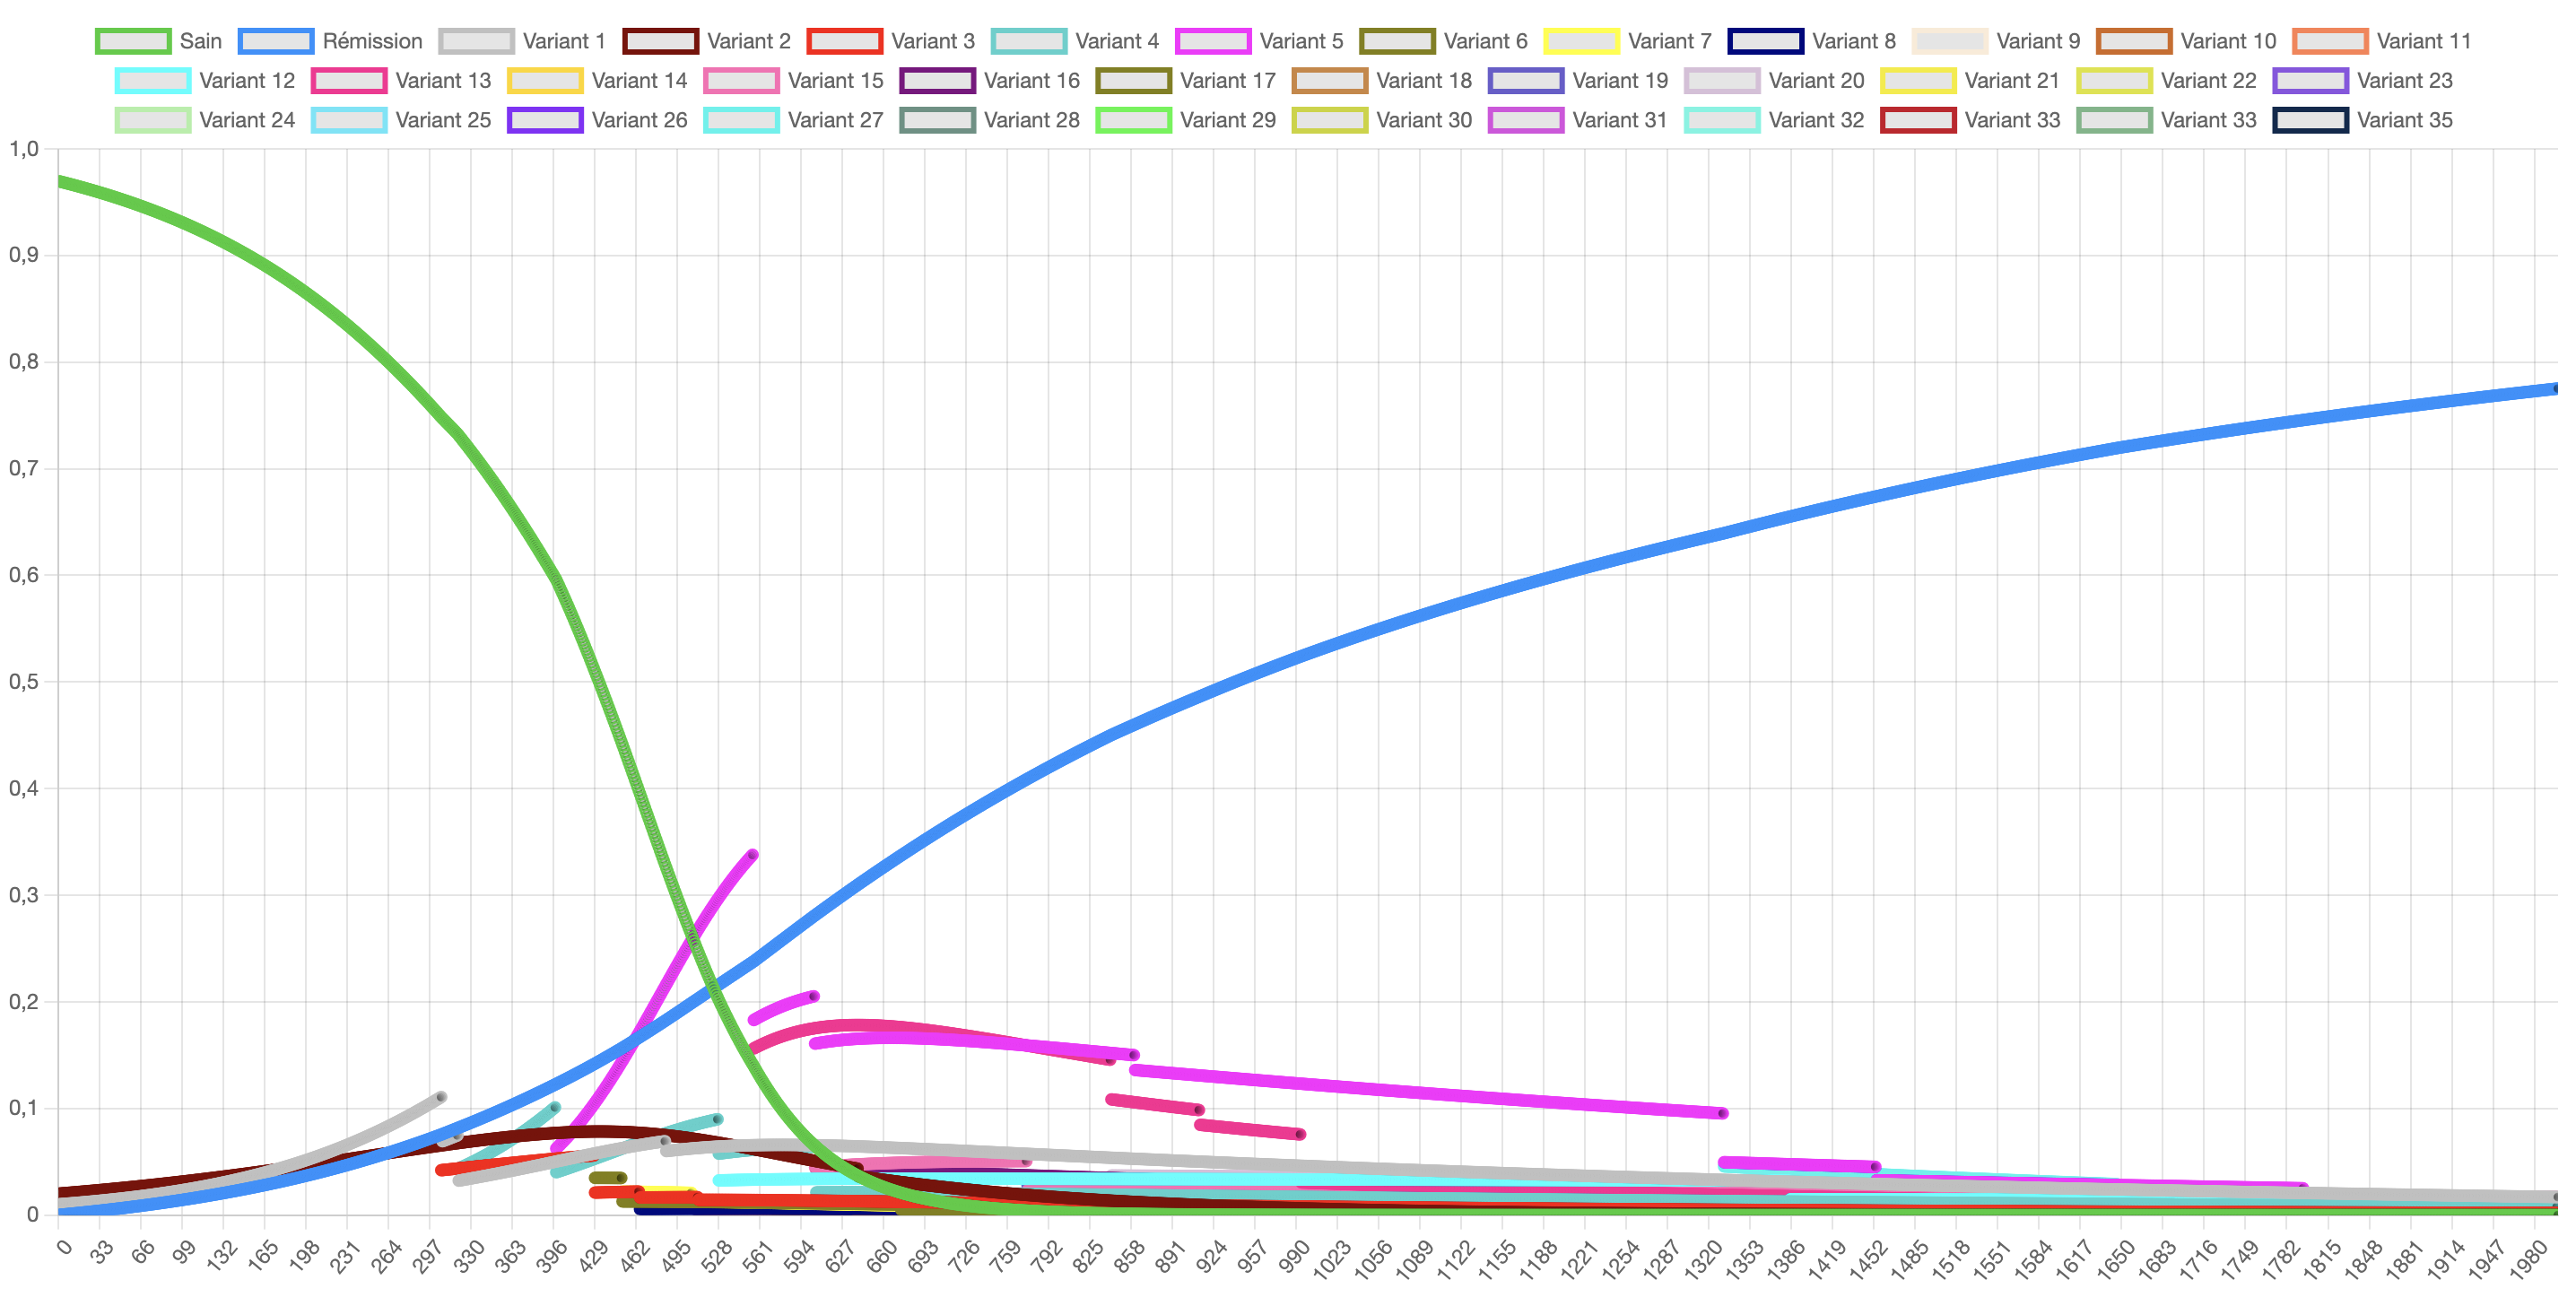
\includegraphics[width=1\linewidth]{images/Simulation2_2.png}
  \caption{Mutabilité du virus plus haute}
  \label{fig:sub2}
\end{subfigure}
\end{figure}

Pour cette simulation, on a décidé de modifier le paramètre suivant :
\begin{enumerate}
    \item Mutabilité du virus = 0,005 pour la figure (a)
    \item Mutabilité du virus = 0,05 pour la figure (b) \\
\end{enumerate}

\noindent
Pour cette simulation, deux simulations ont été faites afin de mettre en avant la modification du paramètre de mutaibilité. Concernant la simulation de la figure 2.a, on remarque la création de seulement 2 variants et la dominance du variant 1. Tandis que pour la simulation de la figure 2.b, on remarque la création de 33 variants mais aucun variant ne prend jamais le dessus sur les autres. Etant donné que lors de la création d'un nouveau variant, ce dernier "vole" une grande partie de la population de son parent, et que la mutabilité est élevée, il n'est pas possible pour un variant de prendre le dessus sur tous les autres.

\subsection{Influence de la force de contagion du premier variant}

\begin{figure}[h]
    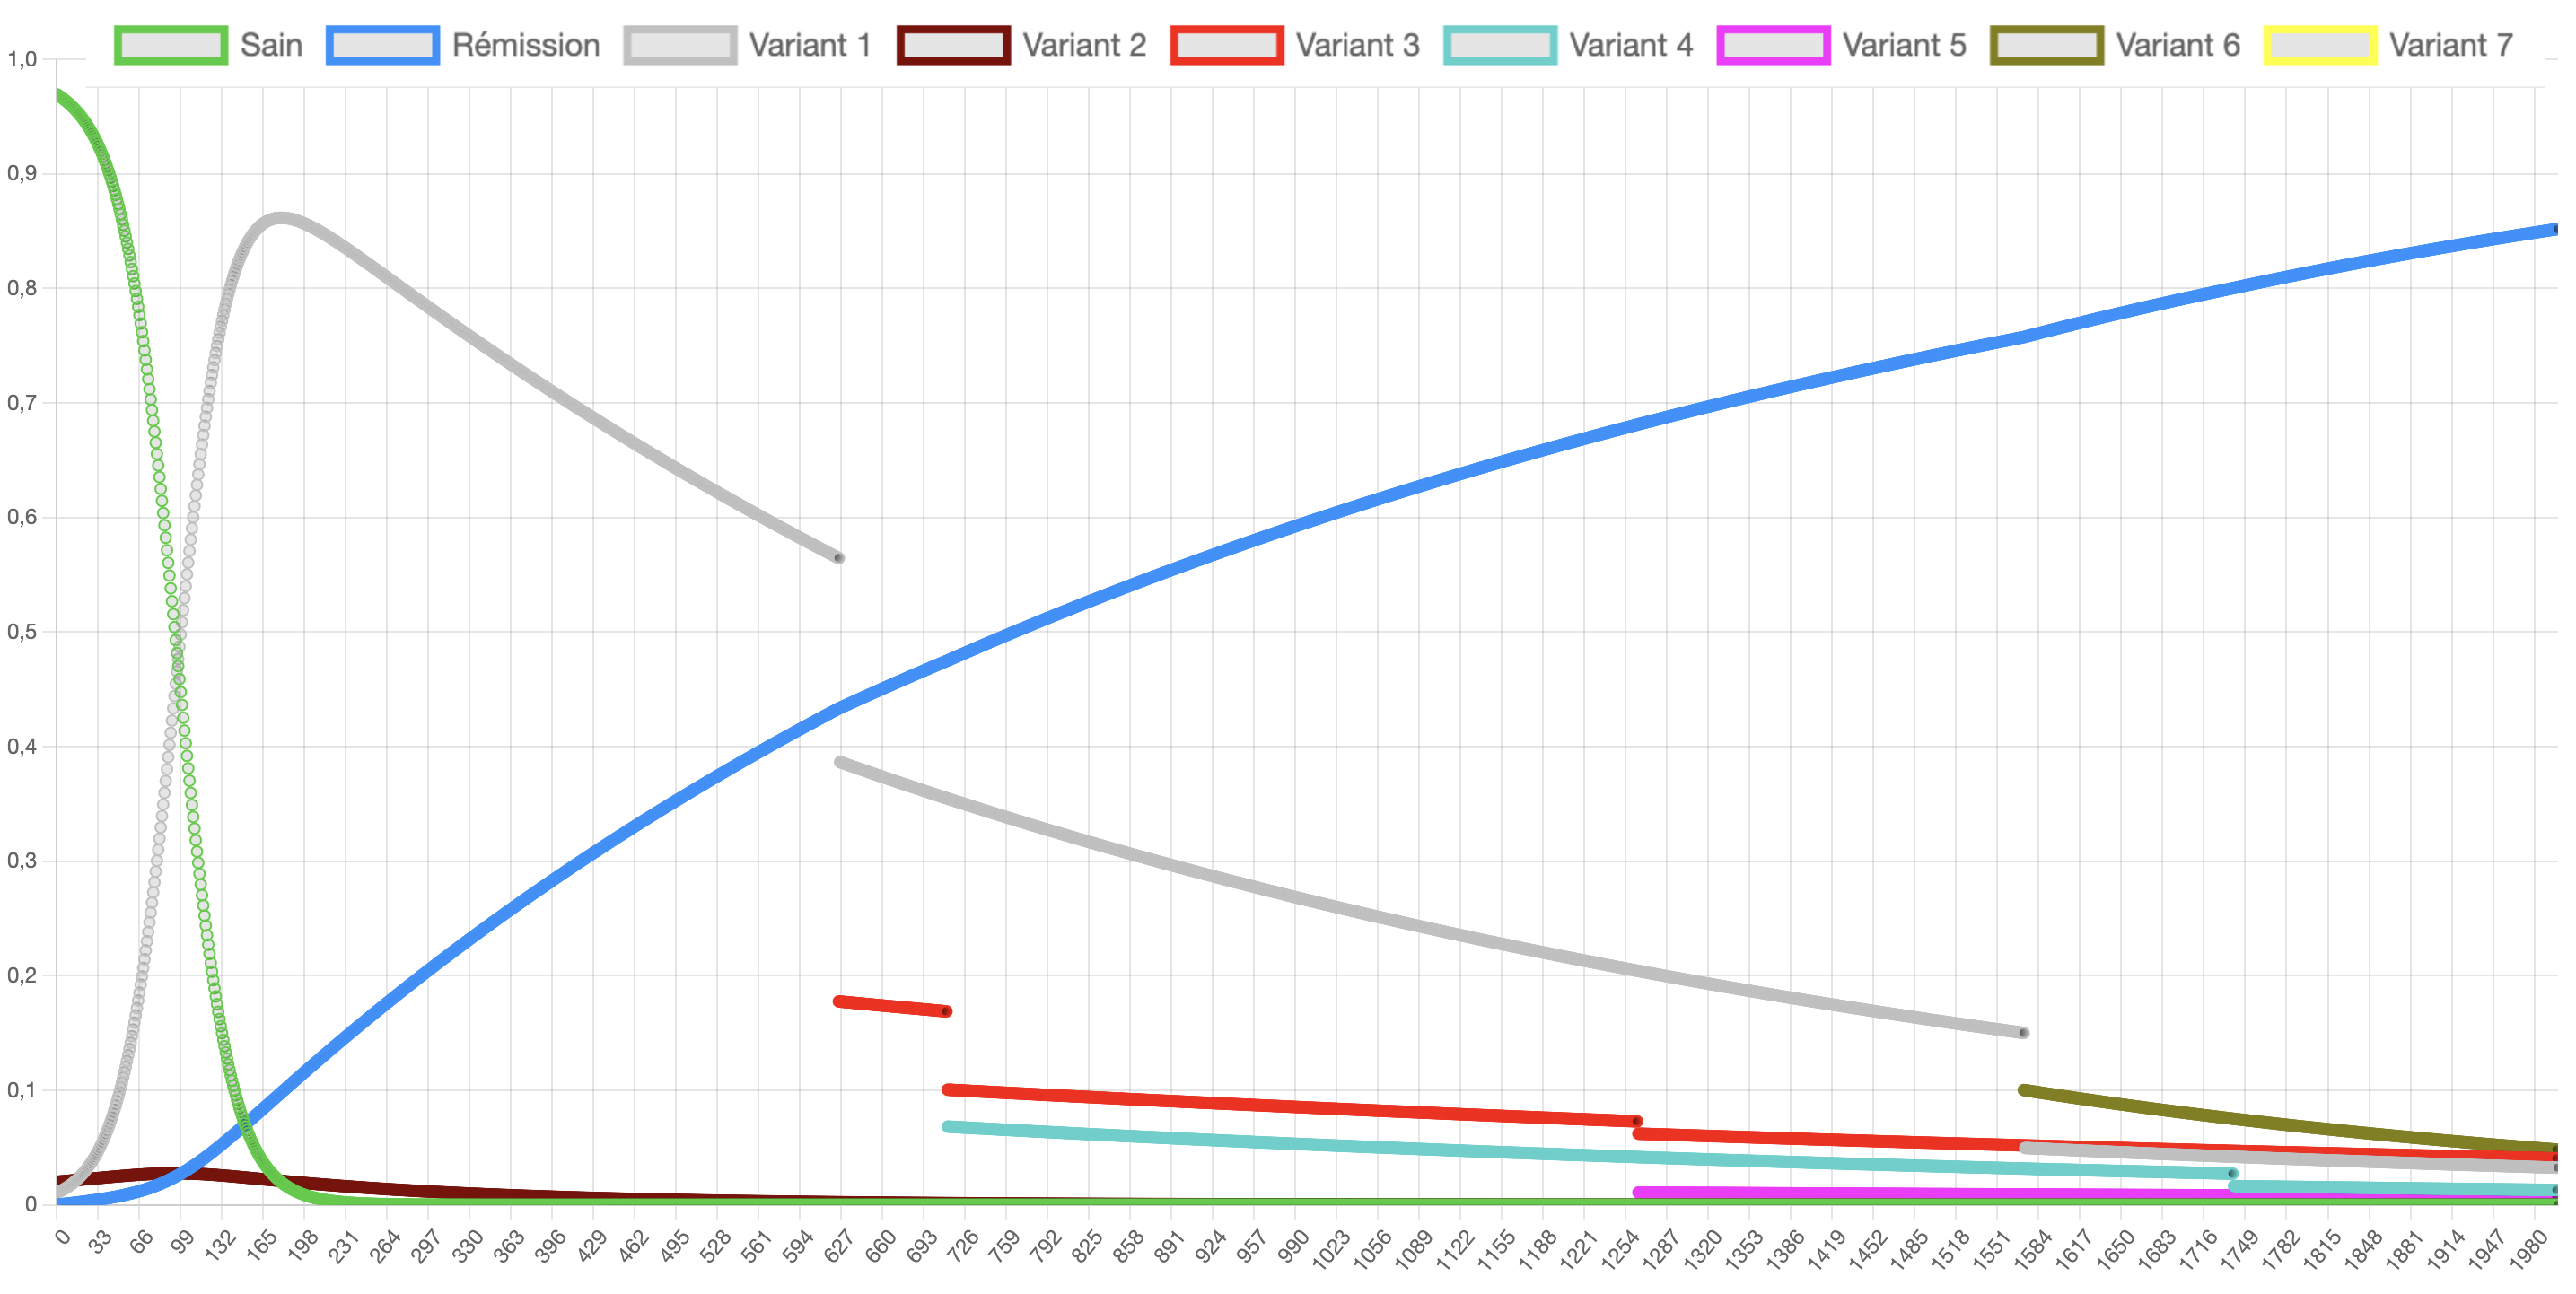
\includegraphics[width=\linewidth]{images/Simulation3.png}
    \caption{Influence de la force de contagion}
    \label{fig:simulation3}
\end{figure}

Pour cette simulation, on a décidé de modifier le paramètre suivant :
\begin{enumerate}
    \item Force de contagion du variant 1 (quantité de virus / mL) = 0,05 \\
\end{enumerate}

\noindent
On remarque qu'avec un taux de contagion plus élevé, le variant 1 infecte jusqu'à presque 90\% de la population très rapidement et devient, par conséquent, le parent ou grand-parent de tous les variants. Le variant 2 quant à lui n'infecte quasiment aucune de la population et disparaît très rapidement. \\

\subsection{Influence de la virulence du premier variant}

\begin{figure}[h]
    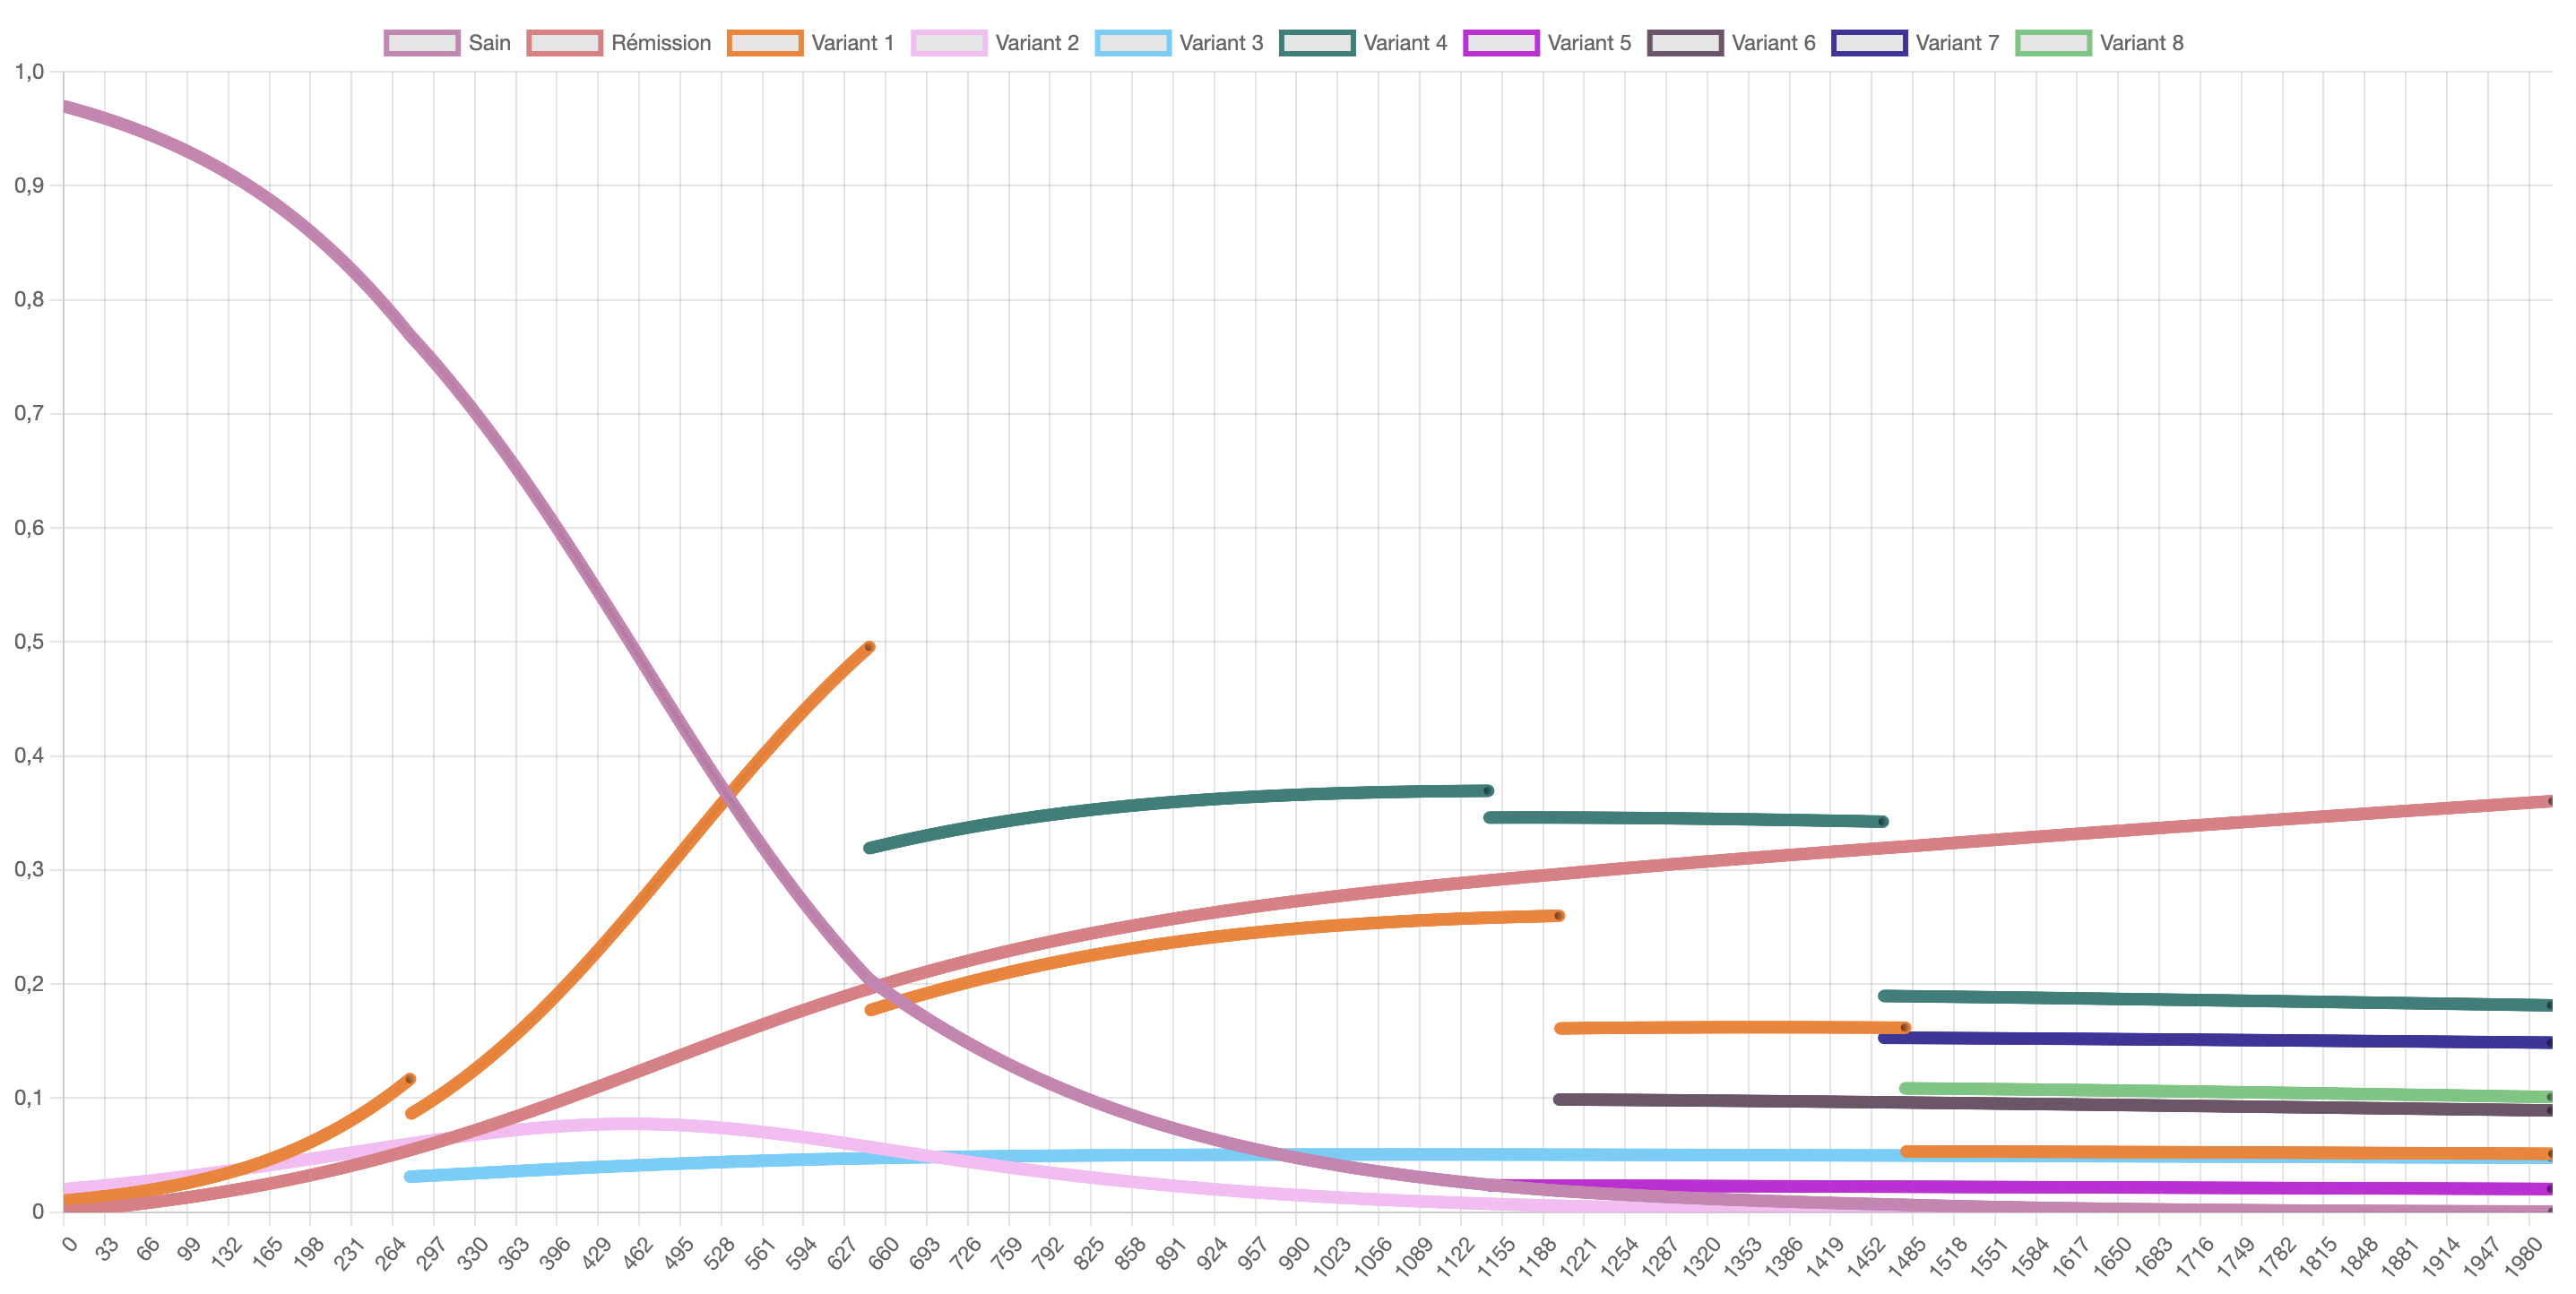
\includegraphics[width=\linewidth]{images/Simulation4.png}
    \caption{Influence de la virulence du premier variant}
    \label{fig:simulation4}
\end{figure}

Pour cette simulation, on a décidé de modifier le paramètre suivant :
\begin{enumerate}
    \item Virulence du variant 1 (\% de survie) = 0,0001 \\
\end{enumerate}

\noindent
On remarque qu'avec un taux de virulence plus faible qui entraine une virulence plus forte, le variant 1 infecte quasiment toute la population et le taux de rémission reste faible après 2000 jours. \\ Cependant, en observant la tendance de la courbe du taux de rémission, on se rend compte que si l'on double le temps de la simulation, le taux de rémission arrivera à 1.
Enfin, on remarque que la plupart des variants (Variant 4, 5, 7, 8, 10) sont plus forts que le variant parent à la fin de la simulation. \\

\subsection{Simulation pour avoir un variant gagnant sur le taux de rémission}

\begin{figure}[h]
    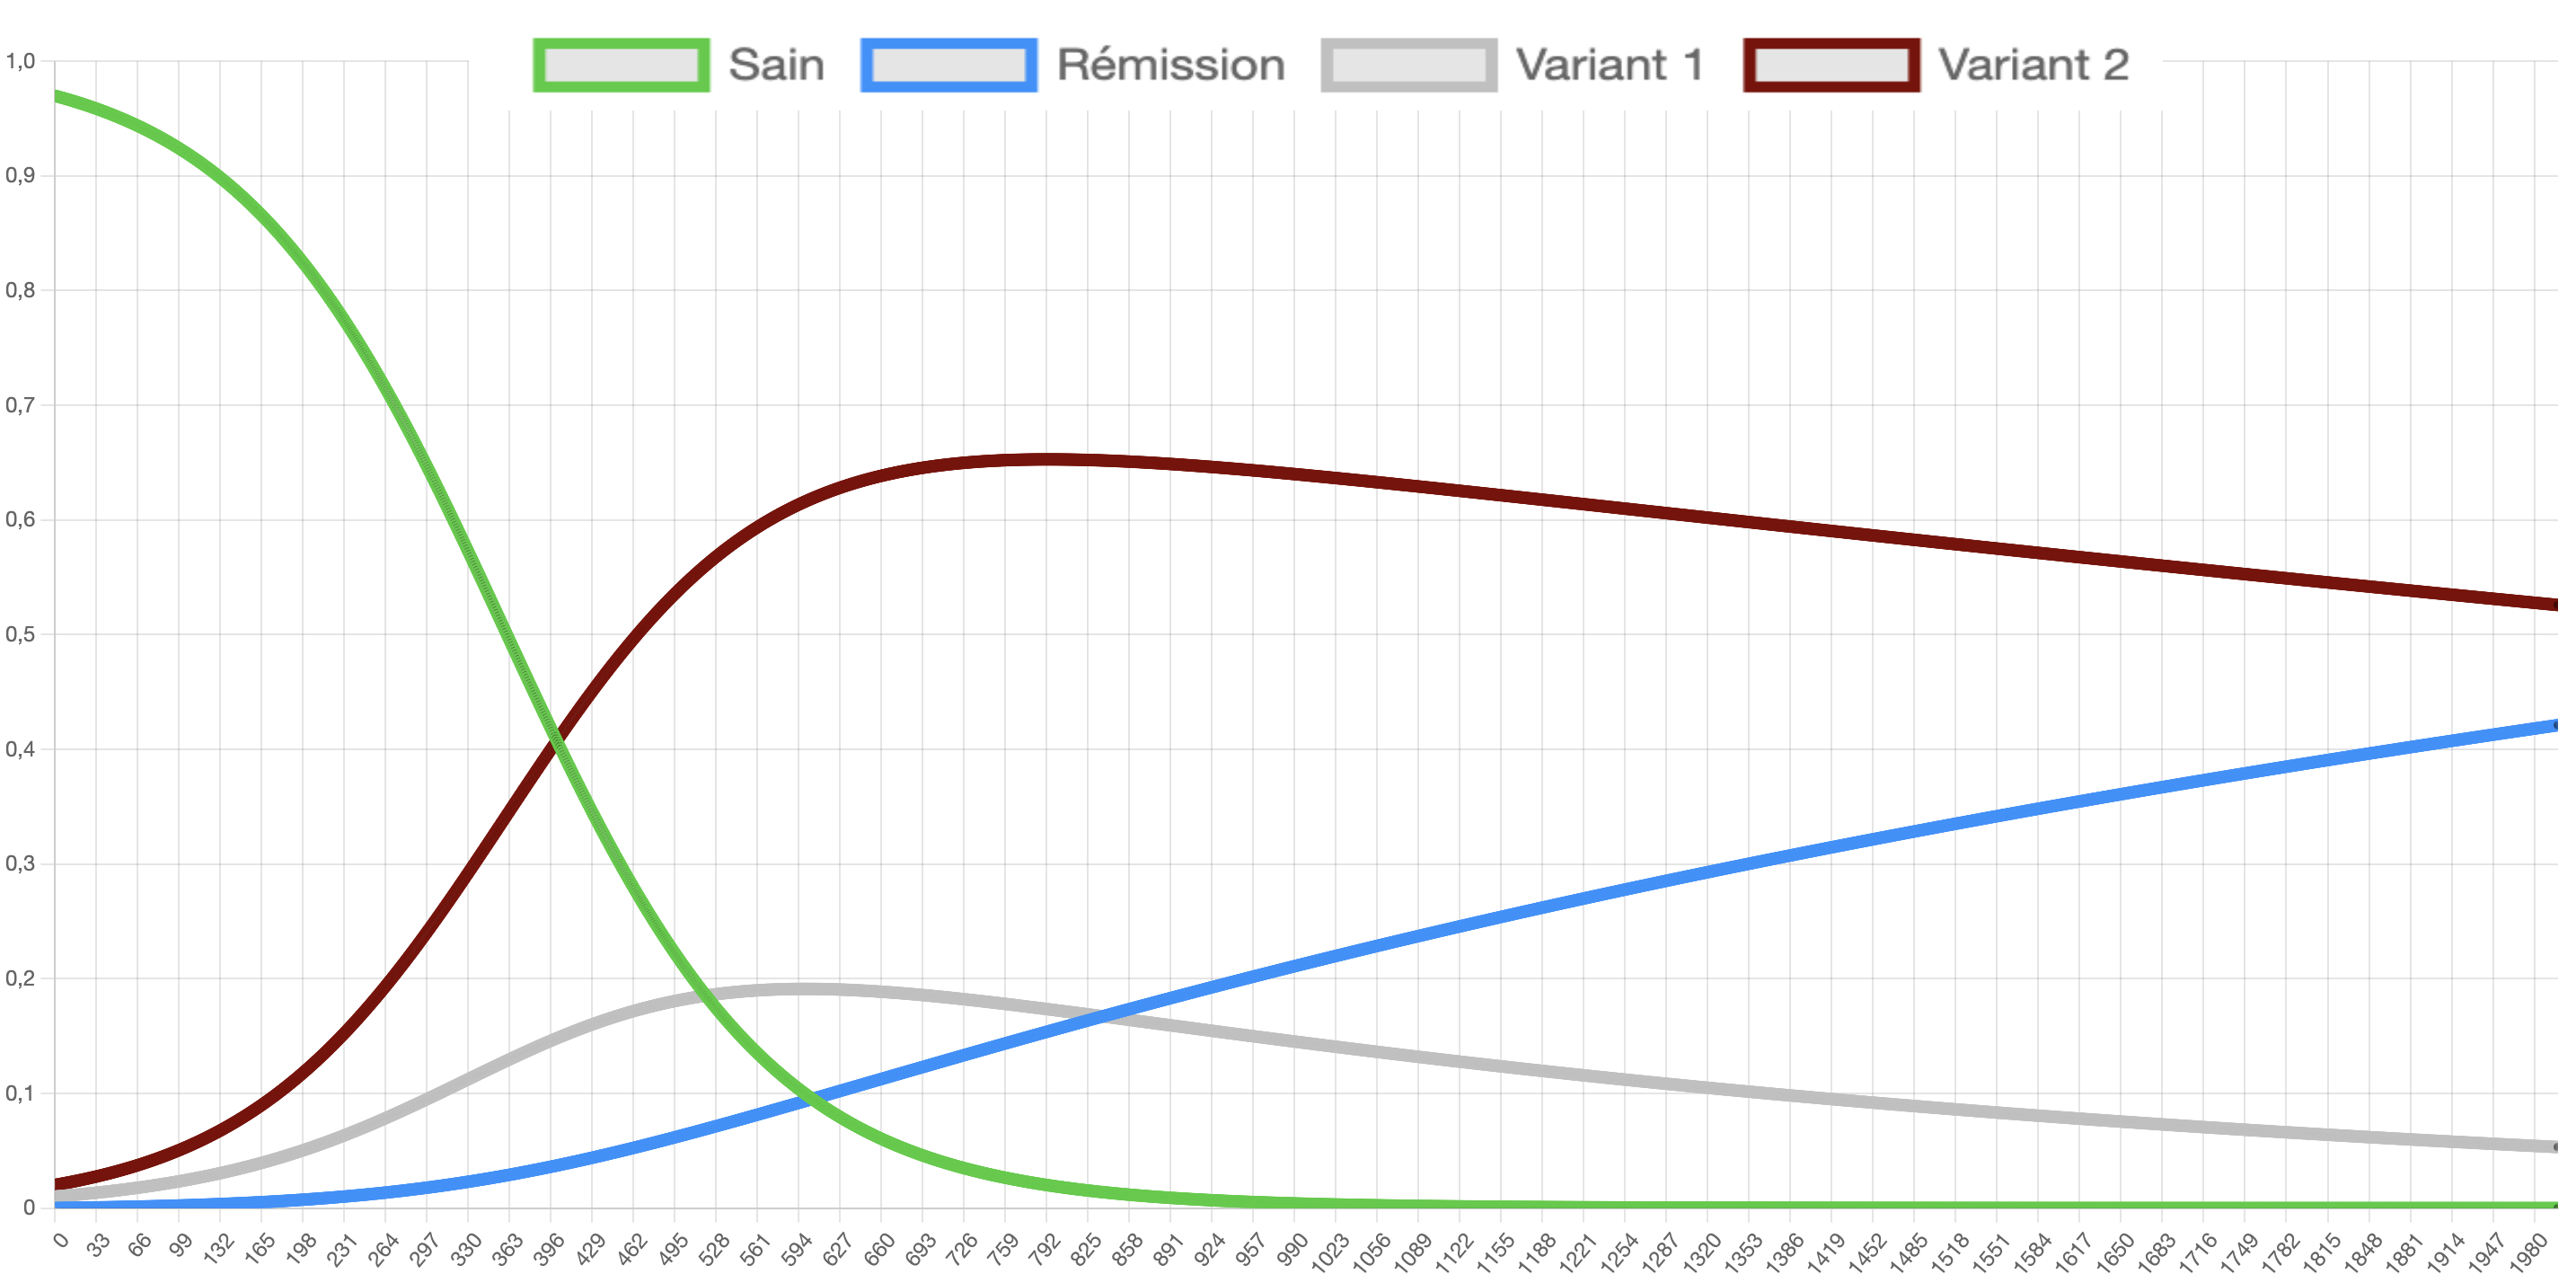
\includegraphics[width=\linewidth]{images/Simulation5.png}
    \caption{Simulation pour avoir un variant gagnant sur le taux de rémission}
    \label{fig:simulation5}
\end{figure}

Pour cette simulation, on a décidé de modifier les paramètres suivants :
\begin{enumerate}
    \item Mutabilité du virus = 0,0001
    \item Virulence du variant 2 (\% de survie) = 0,0002
\end{enumerate}
\noindent
Durant cette simulation, nous avons modifié plusieurs paramètres afin d'arriver à un résultat voulu : avoir un variant avec un taux d'infectés supérieurs au taux de rémission. On a donc modifié la mutabilité du virus afin d'éviter la création de variant et d'entraîner la chute des variants de base. De plus, on a altéré la virulence du variant 2 afin qu'il soit plus fort. On remarque donc qu'à la fin de la simulation, on a le résultat voulu. Cependant, on peut être sûr que si la simulation avait duré plus longtemps, le taux de rémission serait devenu majoritaire.


\section{Discussion des résultats}

\begin{figure}[h]
    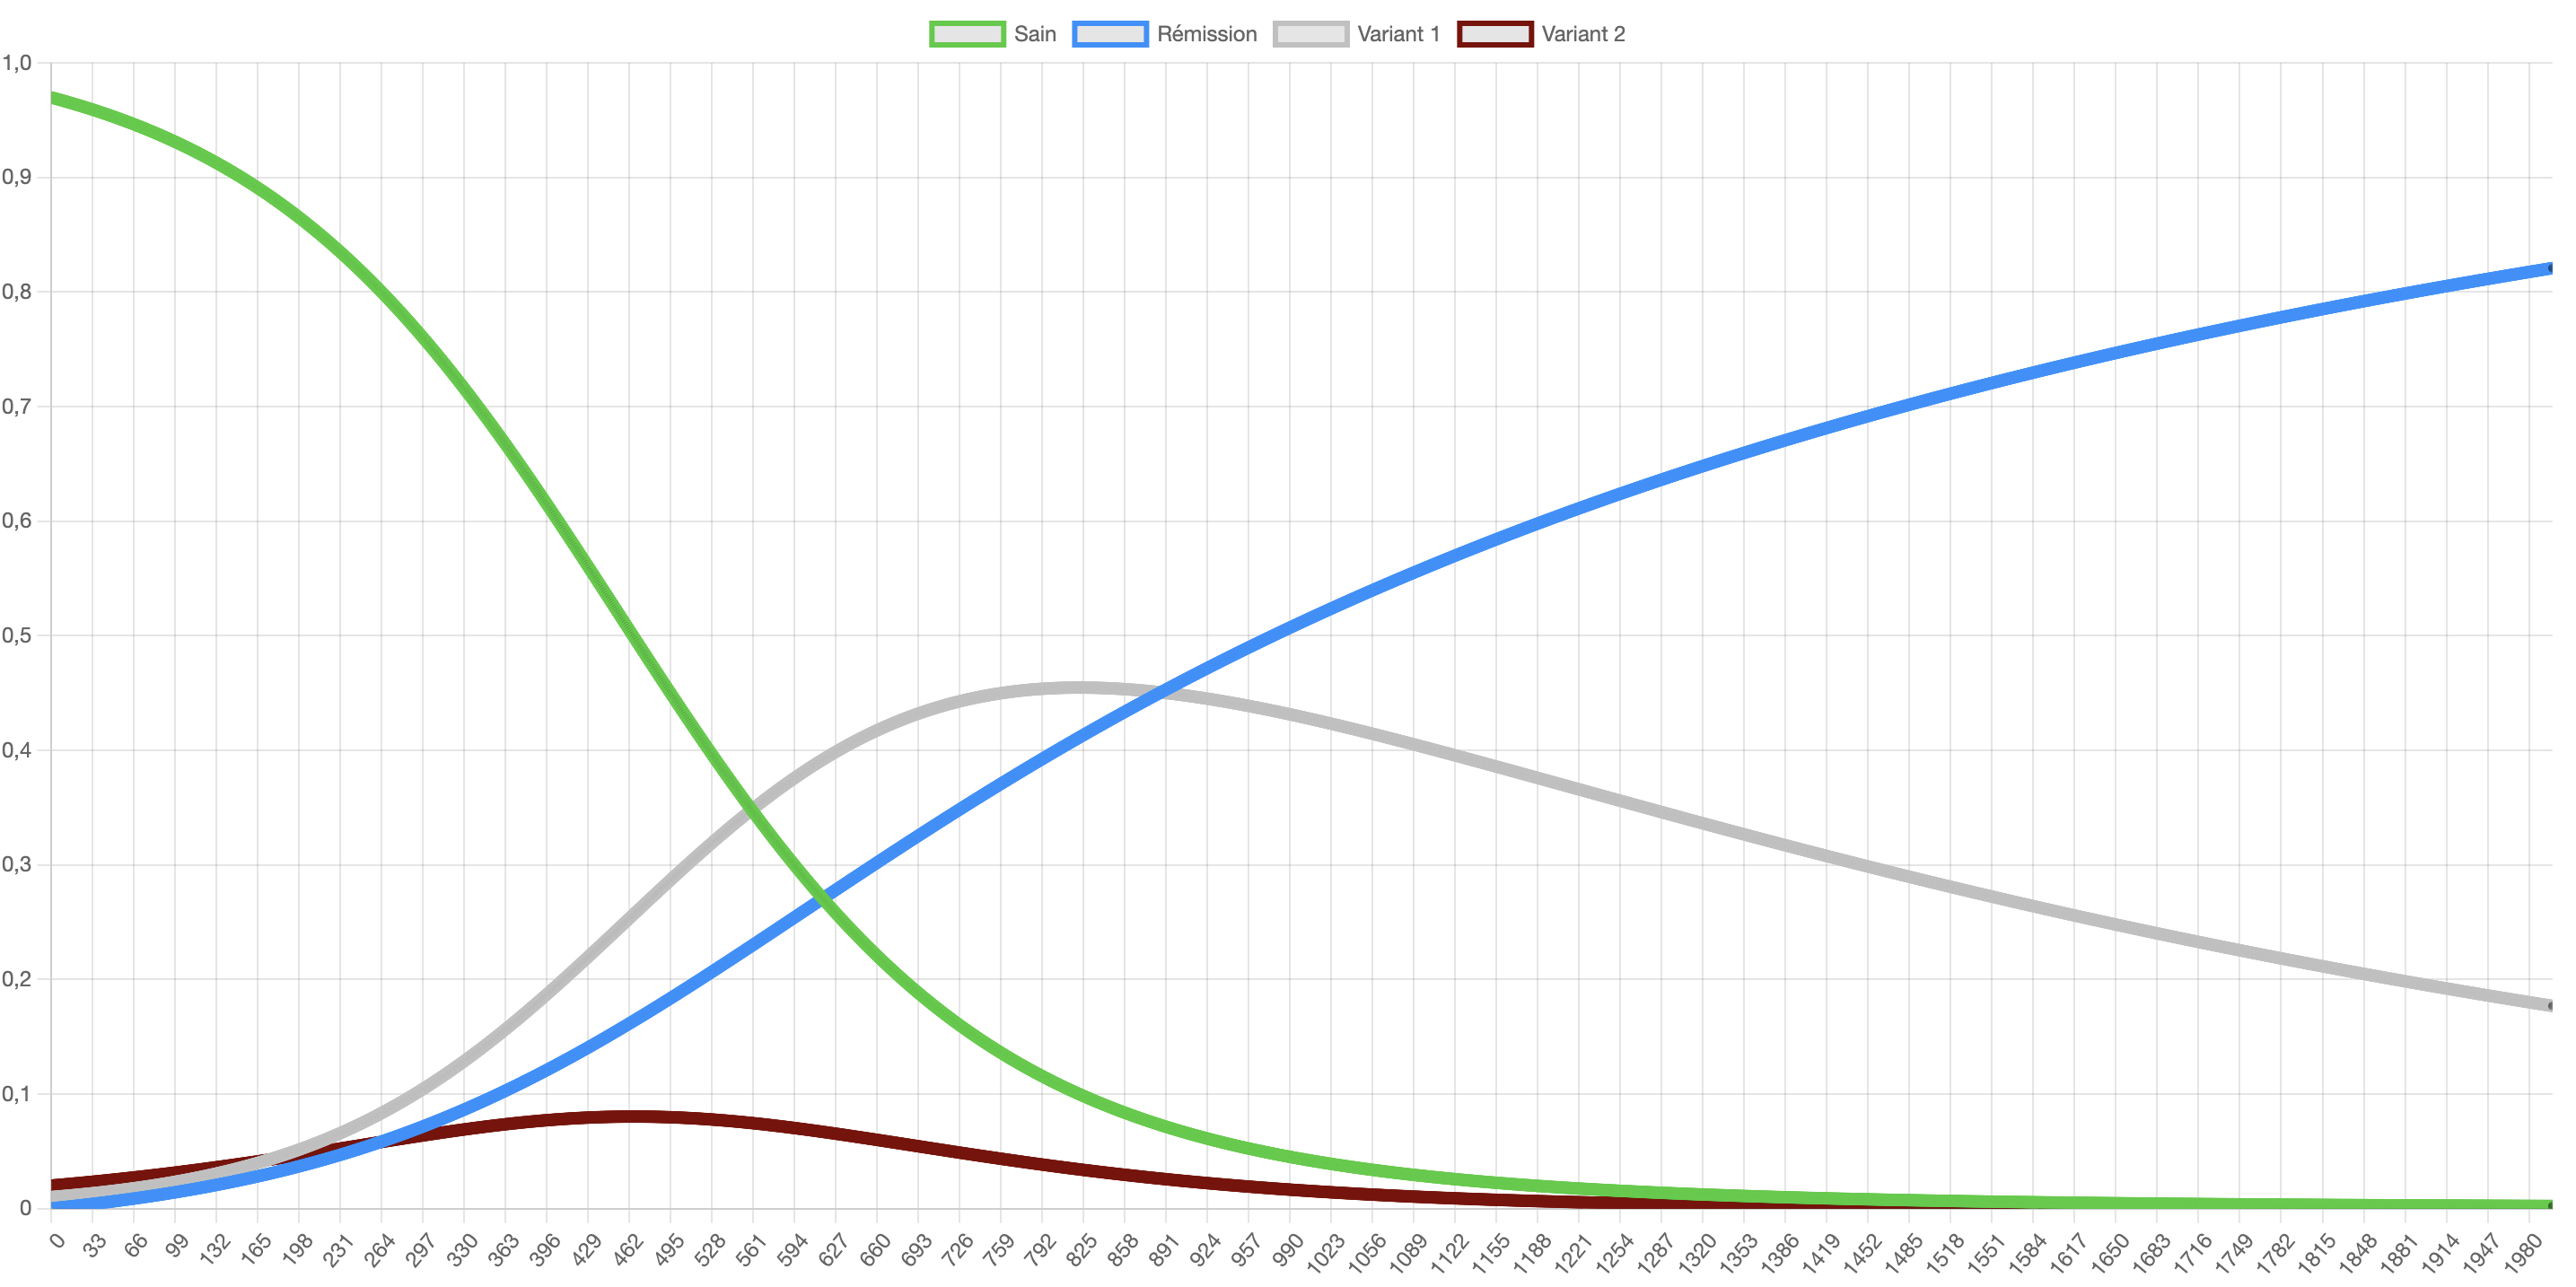
\includegraphics[width=\linewidth]{images/Simulation6.png}
    \caption{Simulation avec les variants initiaux (Mutabilité du virus = 0,0001)}
    \label{fig:simulation6}
\end{figure}


Dans cette partie, nous allons comparer nos différentes simulations à la simulation de la figure 6 qui représente notre modèle sans création de nouveaux variants. Tout d'abord, sur la simulation 6, on peut noter que le variant 1 prend le dessus grâce à sa plus forte virulence. C'est un effet que l'on peut confirmer grâce à la simulation 4 (Influence de la virulence du premier variant). De plus, pour obtenir une simulation avec peu ou pas de nouveaux variants, il faut diminuer la mutabilité du virus, avec la simulation 2 (Influence de la mutabilité du virus), on a pu confirmer cette affirmation. Ensuite, on remarque que le variant 1 à une plus faible force de contagion que le variant 2 mais que pourtant, il prend rapidement le dessus. On a pu observer cet effet de la contagion dans la simulation 3 (Influence de la force de contagion du premier variant). Certes, le variant 1 infecte une grande partie de la population rapidement, mais il ne reste que très peu de temps dominant. La contagion n'est donc pas un critère très important à moins d'être combiné avec d'autres paramètres. Et enfin, on remarque que la virulence du variant est un critère très important, en effet, la simulation 5 et 6 ont un taux de mutabilité égal, cependant pour la simulation 6 aucun variant ne domine à la fin de simulation tandis que pour la simulation 5 (Simulation pour avoir un variant gagnant sur le tauxde rémission), le variant 2 domine car il a une virulence plus forte, même si étant donné que la population ne baisse pas (le décès n'est pas modélisé), cette dernière ne peut donc que se remettre. Ainsi, avec une durée "infinie", on obtient un taux de rémission toujours revenu à la totalité de la population. \\

\section{Conclusion}

Le comportement de l'épidémie de la COVID-19 est-il influencé par la circulation, la mutation et l'interaction des variants ?
À partir des différentes simulations réalisées, il a été conclu que si l'on combine une forte circulation d'un variant ou une forte virulence avec un taux de mutabilité élevé alors un virus pouvait rapidement infecter la quasi-totalité de la population initiale. De plus, l'interaction entre les variants permet de voir que si la virulence d'un variant est forte alors un variant enfant peut contaminer plus de monde à l'inverse de son parent qui contaminera donc bien moins de personnes, étant donné que la population d'un variant enfant provient de la population infectée de son parent. \\
\noindent
Concernant les perspectives d'améliorations, nous pouvons envisager :
\begin{enumerate}
    \item La gestion du nombre de variants de départ. Cela permettrait d'approfondir encore plus les possibilités de simulation.
    \item L'ajout d'une notion de graine liée au randomisateur. Avec cela, on peut s'assurer que les résultats obtenus sont toujours identiques pour les mêmes paramètres bien que l'on utilise un système se basant sur une forme d'aléatoire.
    \item La possibilité de se faire infecter par plusieurs variants en même temps. (il pourrait être intéressant d'intégrer des paramètres plus biologiques au variant afin de créer de la compétition dans le corps des infectés.)
    \item La possibilité de se faire infecter une nouvelle fois après guérison d'un autre variant.
    \item L'ajout d'une notion de vaccination, les personnes saines pourraient être vaccinées ou non ainsi que les personnes remises.
    \item Ajouter des détails au moment de la création d'un variant (notamment sur le fait de savoir s'il est né avec des paramètres très différents de son parent).
    \item Enfin, il manque une notion principale, le fait de pouvoir décéder du variant. Dans nos simulations, la population est soit saine, soit en rémission soit infectée mais elle ne peut pas être infectée puis décédée.
\end{enumerate}

\section{Référence}

Marquioni, V., & de Aguiar, M. (2021). Modeling neutral viral mutations in the spread of SARS-CoV-2 epidemics. PLOS ONE, 16(7), e0255438. doi: 10.1371/journal.pone.0255438


\end{document}
